\section{Costumer overview}
The problem in attaining broad coverage of use cases, and therefore completeness in requirements i primarily that, from the customer perspective, that they feel very overly-verbose and usually too formal in nature. For software engineers, the opposite is usually the case. They feel that the use case descriptions are not structured nor elaborate enough for use in, for instance, code stub generation.

More structure, however, could be helped along the way with proper tooling. Hiding some of the complexity of the constrains of a data model behind a simple user interface supplying dragable components and providing immediate visual feedback in the form of textual use case representation (or a diagram) could "cheat" the customer into adding the needed structure to the use case model.

\begin{figure}[h]
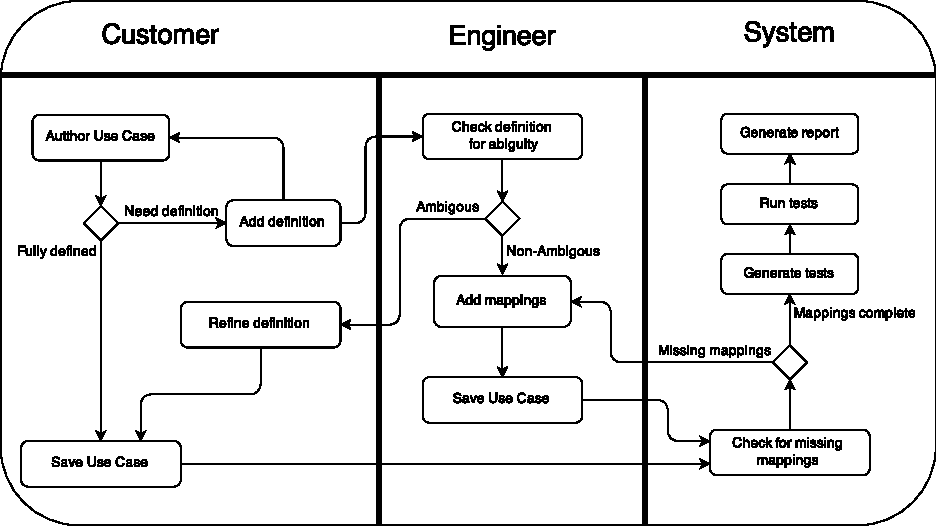
\includegraphics[scale=0.75]{img/use_case_creation_activity_diagram}
\centering
\caption{Use case creation with different actors}
\label{fig:use_case_creation_activity_diagram}
\end{figure}

What is in the customers interest is having acceptance tests match the use cases as closely as possible. Preferably, the should be able to be automated as well. Figure \ref{fig:use_case_creation_activity_diagram} shows an activity diagram involving three actors, the customer, the engineer and the system\footnote{Use case system}. In this diagram, the customer authors use cases while adding missing definitions not already in the tool. A definition is textual description of a concept which may be -- for instance -- an actor, role or action. This description is then given a unique name, that may correspond to a concept already found in the domain model. The domain model, if defined beforehand, could also be thought to be a part of the built-in declarations.

\begin{figure}[h]
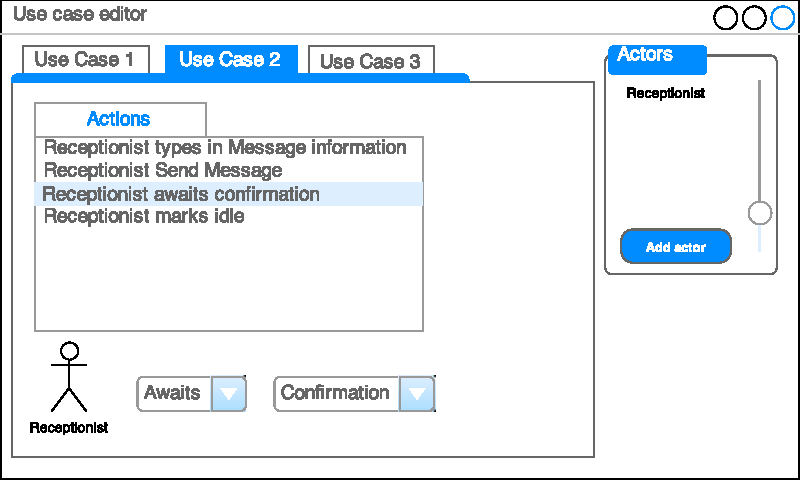
\includegraphics[scale=0.9]{img/test_case_ui}
\centering
\caption{Use case editor UI mockup}
\label{fig:use_case_editor_mockup}
\end{figure}

Whenever there is a new use case, a change to an existing use case, or simply a definition, the system should try to generate tests from the new information. If this step fails it is likely due to insufficient concept mappings. From here, a software engineer must manually map individual definitions to system macro-functionality or, possibly the use case could be linked to an existing manually written test, if the generation step is not possible for some reason. A mockup of a user interface from the customer point of view is shown in figure \ref{fig:use_case_editor_mockup}. A list of available actors (only containing one element, however) is shown on the right hand side. The main part of the window contains the use case currently being worked on. The bottom part of the window is the edit part, where dropdown lists of actions and targets resides.
